\documentclass[UTF8]{ctexart}

\usepackage{geometry}
\geometry{left=3.18cm,right=3.18cm,top=2.54cm,bottom=2.54cm}
\usepackage{graphicx}

% 超链接
\usepackage{hyperref}
\hypersetup{
    hidelinks,
	colorlinks=true,
	allcolors=black,
	pdfstartview=Fit,
	breaklinks=true
}

\usepackage{listings}
\lstset{
    columns=fixed,       
    numbers=left,                                        % 在左侧显示行号
    numberstyle=\tiny\color{gray},                       % 设定行号格式
    frame=none,                                          % 不显示背景边框
    backgroundcolor=\color[RGB]{245,245,244},            % 设定背景颜色
    keywordstyle=\color[RGB]{40,40,255},                 % 设定关键字颜色
    numberstyle=\footnotesize\color[RGB]{40,40,255},           
    commentstyle=\it\color[RGB]{0,96,96},                % 设置代码注释的格式
    stringstyle=\rmfamily\slshape\color[RGB]{128,0,0},   % 设置字符串格式
    showstringspaces=false,                              % 不显示字符串中的空格
	breaklines      =   true,							 % 自动换行
    language=bash,                                       % 设置语言
	columns         =   fixed,
    basicstyle=\setmainfont{Courier New}
}

\title{对 NGS 数据的 ChIP-Seq 分析}
\author{生信2001张子栋}
\date{\today}

% 设置目录显示的深度
\setcounter{tocdepth}{3}

% 设置标号深度
\setcounter{secnumdepth}{3}

% 去除页码 	
\usepackage{setspace}

\begin{document}

\maketitle
\thispagestyle{empty}

\clearpage

\thispagestyle{empty}
\setcounter{page}{0}

\begin{abstract}
    ChIP-seq 有助于了解基因之间的相互调控、表观遗传机制和染色体的结构与动态;可以确定转录因子的结合位点、作用通路、结合 motif 等。可以使用 R 中的一些专门的包来进行 ChIP-seq 数据的peak annotation 和可视化等步骤。参考的数据文章\cite{ref1}使用 ChIP-Seq 的目的是为了发现 HIF-1 直接调控的基因,并分析它们在缺氧应答通路中的功能。
\end{abstract}

\begin{figure}[!htb]
	\centering
	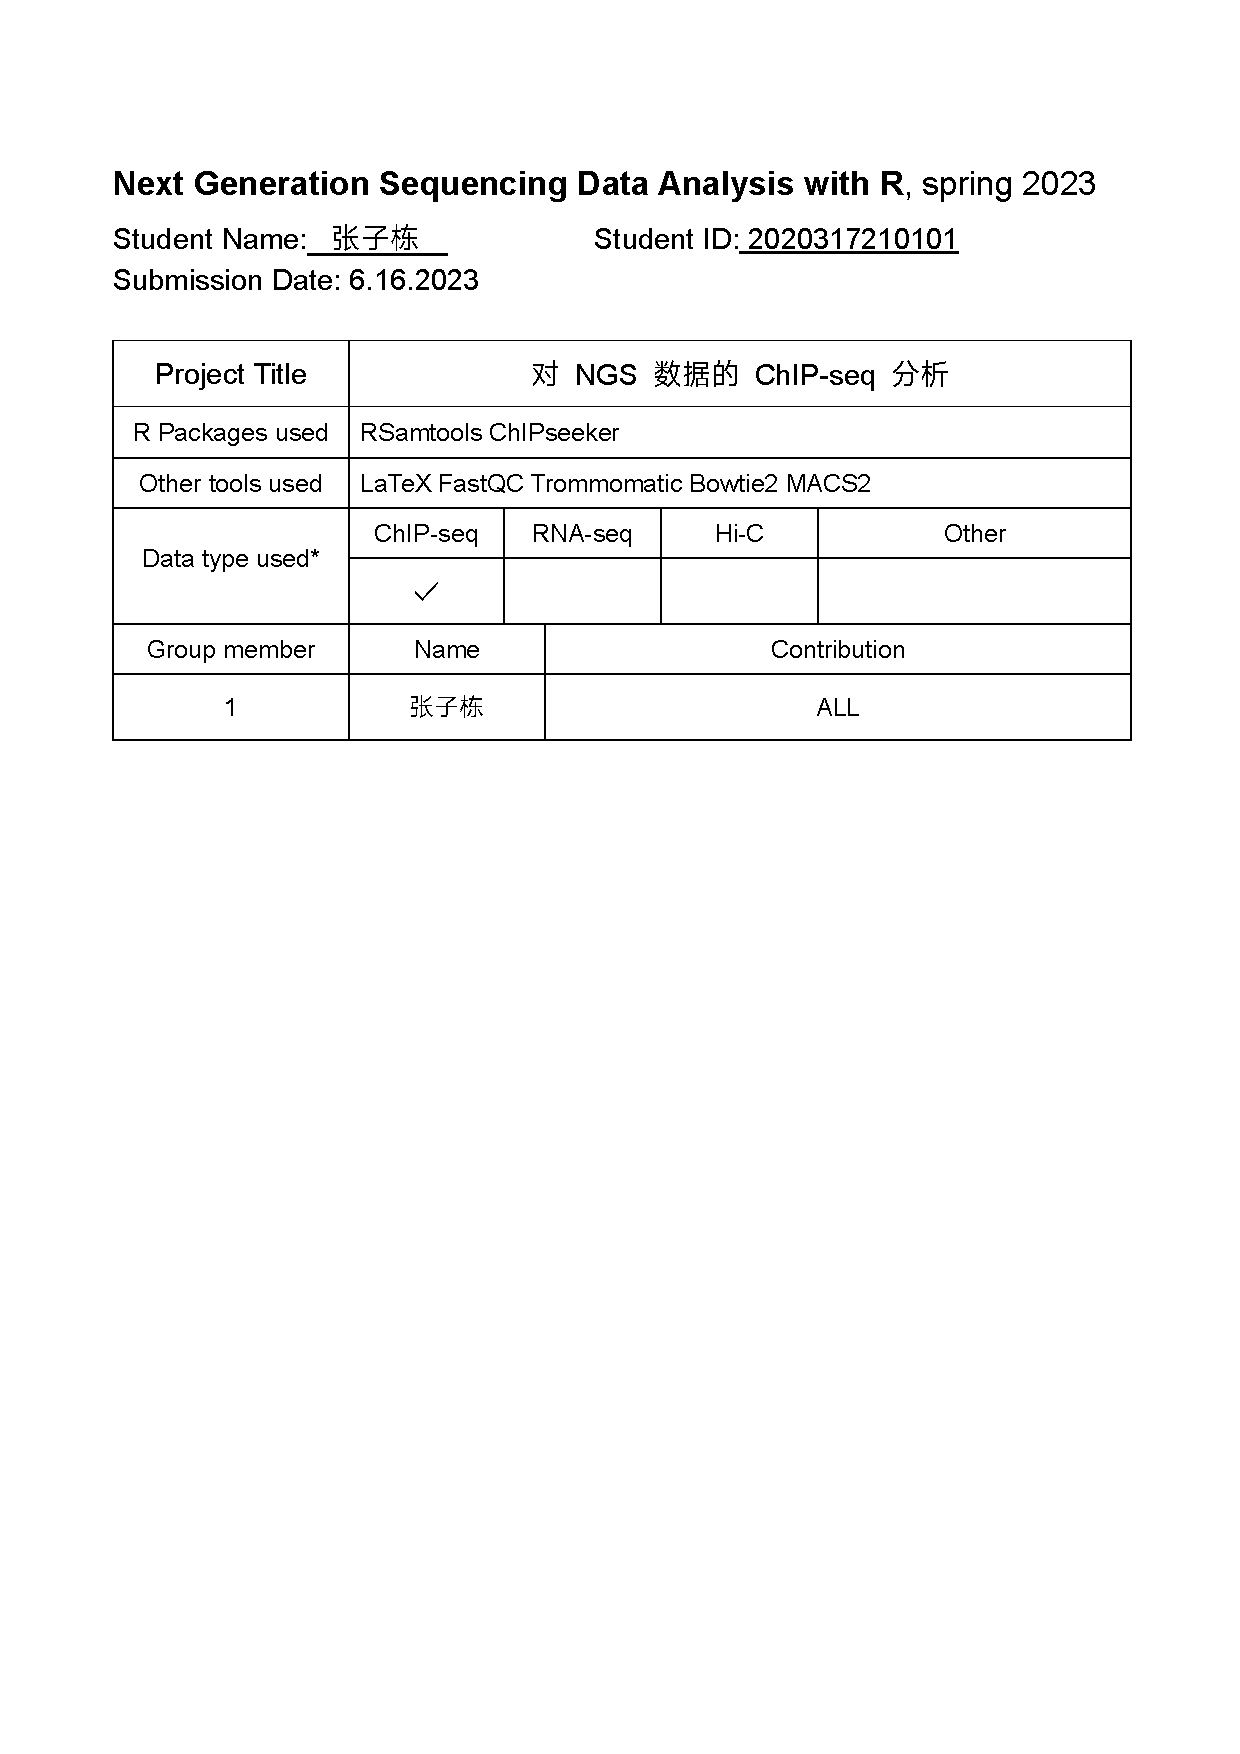
\includegraphics[width=\textwidth]{img/Final_project_cover.pdf}
\end{figure}

\clearpage

\thispagestyle{empty}
\tableofcontents
\setcounter{page}{0}

\clearpage

\section{项目材料及目的}

\subsection{PubMed 数据库中搜索数据文献}

\subsubsection{选定研究物种}

选定研究物种为线虫($nematode,\ Caenorhabditis\ Elegans$)。

\subsubsection{在 PubMed 中检索文献}

在 \href{https://pubmed.ncbi.nlm.nih.gov/}{PubMed (nih.gov)} 中搜索关键字 Caenorhabditis Elegans ChIP-seq. 并选定文献为 \href{https://pubmed.ncbi.nlm.nih.gov/36257965/}{The hypoxia response pathway promotes PEP carboxykinase and gluconeogenesis in C. elegans} (Nat Commun. 2022 Oct 18;13(1):6168. DOI: \href{https://doi.org/10.1038/s41467-022-33849-x}{10.1038/s41467-022-33849-x} )\cite{ref1}.

这篇文章研究的内容是在线虫中,缺氧应答通路如何通过激活 HIF-1 转录因子来调节 PEP 羧激酶和糖异生的基因表达和代谢流动,从而提高对氧化应激和缺氧应激的抵抗力。PEP 羧激酶是糖异生过程中的限速酶,可以将草酰乙酸转化为磷酸烯醇式丙酮酸。

作者利用基因组编辑、转录组分析、代谢组分析和行为实验等方法来揭示 HIF-1 直接或间接调控的上百个基因的功能。这篇文章使用 ChIP-Seq 的目的是为了发现 HIF-1 直接调控的基因,并分析它们在缺氧应答通路中的功能。

\section{数据与方法}

\subsection{NGS 数据获取}

文章中的 ChIP-seq 数据上传至 NIH/NCBI 数据库,登录号为 \href{https://www.ncbi.nlm.nih.gov/geo/query/acc.cgi?acc=GSE173333}{GSE173333}。SRA 数据库对应登录号为 \href{https://www.ncbi.nlm.nih.gov/sra?term=SRP316378}{SRP316378} ,并最终选择 SRR14325856 和 SRR14325854作为研究数据。

使用以下命令下载数据:

\begin{lstlisting}
wget https://trace.ncbi.nlm.nih.gov/Traces/sra-reads-be/fastq?acc=SRR14325856
\end{lstlisting}

\subsection{线虫参考基因组}

\subsubsection{WormBase}

WormBase 是一个专门收录线虫的基因组信息的数据库,它支持使用线虫作为模式生物的研究者,提供了线虫的基因组序列、注释、变异、表达、互作等数据。WormBase 还包括一个子项目WormBase ParaSite,它收录了其他线虫和扁形动物寄生虫的基因组信息。参考基因组是一个完整的线虫基因序列,基因组注释文件是对参考基因组中的基因、转录本、外显子等特征的描述。

通过 \href{https://wormbase.org/}{WormBase : Nematode Information Resource} 网站获取线虫参考基因组。

\subsection{R包及其他软件}

\subsubsection{FastQC}

FastQC 是一个质量控制分析工具,用于检测高通量测序数据中的潜在问题。它提供了一系列的分析模块,可以帮助快速了解数据是否有任何需要注意的问题,以便进行进一步的分析。FastQC 可以处理 fastq 或 bam 格式的原始序列文件,并生成一个报告,总结分析结果。

FastQC 的报告是一个 HTML 文件,包含了各种分析模块的结果和图表。FastQC 的报告中,每个分析模块都有一个结果图和一个状态图标。状态图标表示该模块的结果是否正常(绿色)、需要注意(黄色)或有问题(红色)。

FastQC 有以下几个分析模块:

\begin{itemize}
	\item 基本统计:显示输入文件的名称、编码类型、总读数、读长和 GC 含量等信息。
	\item 每碱基质量分布:显示每个位置的平均质量得分,以及上下四分位数的范围。
	\item 每序列质量分布:显示每个序列的平均质量得分的频率分布,以及对应的合格率。
	\item 每碱基序列内容:显示每个位置的 A、T、G 和 C 的比例,以及与理论值的偏差。
	\item 每序列 GC 含量:显示每个序列的 GC 含量的频率分布,以及与整体 GC 含量的比较。
	\item 每碱基 N 含量:显示每个位置包含 N(未知)碱基的比例。
	\item 序列长度分布:显示不同长度序列出现的频率,以及平均长度和最大长度。
	\item 序列重复度:显示不同重复次数序列出现的频率,以及总重复度和最大重复度。
	\item 过表示 kmer 内容:显示在所有序列中过表达(出现次数超过预期)或者欠表达(出现次数低于预期)的 kmer(一般为 7 或 8 bp),以及它们在序列中出现的位置和比例。
	\item adapter 检测:检测输入文件中是否包含常见 adapter 序列,并显示它们在不同位置出现的比例。
	
\end{itemize}

\paragraph*{FastQC 命令格式}

\begin{lstlisting}
fastqc [-o output dir] [--(no)extract] [-t thread num] [-f fastq|bam|sam] [-c contaminant file] seqfile1.. seqfileN
\end{lstlisting}

\begin{itemize}
	\item 其中:
	\begin{itemize}
		\item \verb|-o| 用来指定输出文件的所在目录。
		\item \verb|--(no)extract| 用来控制是否解压缩输出的 \verb|.zip| 文件。
		\item \verb|-t| 用来选择程序运行的线程数,即同时处理的文件数目。这样可以提高 fastqc 的运行速度,但也会占用更多的内存资源。
		\item \verb|-f| 用来强制指定输入文件格式,默认会自动检测。
		\item \verb|-c| 用来指定污染物文件,用于检测序列中是否含有不期望的序列。
		\item \verb|seqfile1.. seqfileN| 表示可以输入多个序列文件,支持 \verb|fastq, bam| 和 \verb|sam| 格式。
	\end{itemize}
\end{itemize}

\subsubsection{Trommomatic}

Trimmomatic 是一个快速的多线程命令行工具,于 2014 年首次发表在 Bioinformatics 期刊上,它可以用来整理和裁剪 Illumina (FASTQ) 数据以及删除 adapter。

Trimmomatic 有两种过滤模式,分别对应单末端(SE)和双末端(PE)测序数据,同时支持 \verb|gzip| 和 \verb|bzip| 压缩文件。它还支持 \verb|phred-33| 和 \verb|phred-64| 格式互相转化,目前多数 Illumina 测序数据为 \verb|phred-33| 格式。

\begin{itemize}
	\item Trimmomatic 的主要功能包括:
	\begin{itemize}
		\item 去除 adapter 序列以及测序中其他特殊序列。
		\item 采用滑动窗口的方法,切除或者删除低质量碱基。
		\item 去除头(尾)部低质量以及 N 碱基过多的 reads.
		\item 截取固定长度的 reads.
		\item 丢掉小于一定长度的 reads.
		\item phred 质量值转换。
	\end{itemize}
\end{itemize}

\paragraph*{Trimmomatic 命令格式}

Trimmomatic 的命令格式根据使用的是双端模式(PE)还是单端模式(SE)而不同。一般来说,命令格式为:

\begin{lstlisting}
java -jar <trimmomatic.jar> PE|SE [-threads <threads>] [-phred33|-phred64] [-trimlog <logFile>] <input 1> [<input 2>] <output 1> [<output 2>] <step 1> …
\end{lstlisting}

\begin{itemize}
	\item 其中:
	\begin{itemize}
		\item \verb|-jar <trimmomatic.jar>| 是运行 Trimmomatic 的 Java 命令,需要指定\\ \verb|trimmomatic.jar| 文件的路径。
		\item \verb!PE|SE! 如果是双端模式,需要提供两个输入文件和两个输出文件;如果是单端模式,只需要提供一个输入文件和一个输出文件。
		\item \verb|[-threads <threads>]| 是可选参数,用于设置线程数,默认为1。
		\item \verb|[-phred33|-phred64]| 是可选参数,用于设置碱基质量值的编码系统,默认为 phred64。自 v0.32 版本之后,Trimmomatic 可以自动识别是 phred33 还是 phred64。
		\item \verb|[-trimlog <logFile>]| 是可选参数,用于设置日志文件的路径和名称。日志文件记录了每个 reads的修剪情况。 
		\item \verb|<input 1> [<input 2>]| 是输入文件的路径和名称,可以是压缩或非压缩的FASTQ文件。如果是双端模式,需要提供两个输入文件;如果是单端模式,只需要提供一个输入文件。
		\item \verb|<step 1> …| 是指定要执行的修剪步骤和参数。每个步骤之间用空格隔开。目前支持以下几种步骤:
		\begin{itemize}
			\item \verb|ILLUMINACLIP|: 去除接头序列
			\item \verb|SLIDINGWINDOW|: 滑动窗口裁剪低质量碱基
			\item \verb|MAXINFO|: 基于信息熵裁剪低质量碱基
			\item \verb|LEADING|: 去除开头低质量碱基
			\item \verb|TRAILING|: 去除结尾低质量碱基
			\item \verb|CROP|: 裁剪 reads 到指定长度
			\item \verb|HEADCROP|: 去除 reads 开头指定长度
			\item \verb|MINLEN|: 过滤掉小于指定长度的 reads
		\end{itemize}
	\end{itemize}
\end{itemize}

\subsubsection{Bowtie2}

Bowtie 是一个超快的,存储高效的短序列片段比对程序。它能够将短的 DNA 序列片段(reads)比对到人类基因组或其他较大的参考基因组上。它有两个版本:Bowtie 和 Bowtie2。Bowtie2 是 Bowtie 的升级版,能够比对更长的 reads,支持局部比对和剪接性比对。

Bowtie 的使用也需要先对参考基因组建立索引,然后再进行比对。比对的结果是一个 SAM 或 BAM 格式的文件,可以用 Samtools 进行后续的处理。

\subsubsection{RSamtools}

RSamtools 是一个用于处理 SAM 或 BAM 格式的比对结果的软件包,本文使用该 R 包进行比对结果的分析。

\subsubsection{Bedtools}

Bedtools 是一个用于处理基因组数据的软件,它可以对 BED、BAM、GFF 等格式的文件进行各种操作,如求交集、并集、覆盖度、分组统计等。Bedtools 的主要功能有:

\begin{itemize}
	\item \verb|genomecov|:计算基因组的覆盖度,即某些特征覆盖了基因组的哪些部分。
	\item \verb|groupby|:对文件或流按照指定的列进行分组,并对另一列进行统计,类似于数据库的 “group by” 语句。
	\item \verb|intersect|:计算两个文件或流中的特征的交集,即哪些特征在两个文件或流中都存在。
	\item \verb|merge|:合并两个文件或流中的特征,即将有重叠的特征合并为一个特征。
	\item \verb|sort|:对文件或流按照某些列进行排序,以便于其他操作。
\end{itemize}

\subsubsection{MACS2}

MACS是一款用于分析ChIP-seq数据的软件,它可以用来寻找转录因子或组蛋白修饰在基因组上的结合位点。MACS的基本原理是利用ChIP-seq数据中的片段长度和富集度来估计结合位点的位置和显著性。

MACS 的使用需要安装 Python 和一些依赖包,具体的安装方法可以参考官方文档。MACS 的主要命令是\verb|macs2 callpeak|,它可以用来从 ChIP-seq 数据中调用结合位点。基本语法是:

\paragraph*{命令格式}

\begin{lstlisting}
macs2 callpeak -t <ChIP-seq文件> -c <对照文件> -f <文件格式> -g <基因组大小> -n <输出文件名> [其他参数]
\end{lstlisting}

\begin{itemize}
	\item 其中:
	\begin{itemize}
		\item \verb|-t| 和 \verb|-c| 参数分别指定ChIP-seq文件和对照文件,它们可以是BAM, SAM, BED或ELAND格式。
		\item \verb|-f| 参数指定文件格式。
		\item \verb|-g| 参数指定基因组大小
		\item \verb|text| 参数指定输出文件名
		\item 其他参数可以根据需要调整,例如 \verb|text| 参数可以设置p值阈值,\verb|-B| 参数可以输出bedGraph格式的信号强度文件等。
	\end{itemize}
\end{itemize}

\subsubsection{MEME}

MEME是一款用于分析蛋白质,DNA和RNA中的序列Motif的软件,它可以用来寻找转录因子结合位点的共有序列特征。MEME的基本原理是利用最大期望算法(Expectation Maximization)来从一组序列中识别出重复出现的Motif。MEME提供了在线版和本地版。

\paragraph*{命令格式:}
\begin{lstlisting}
meme <序列文件> -o <输出目录> [其他参数]	
\end{lstlisting}

\begin{itemize}
	\item 其中:
	\begin{itemize}
		\item <序列文件>指定输入的序列文件,它可以是FASTA格式或MEME格式。
		\item <输出目录>指定输出结果的目录,它必须不存在或为空。
		\item 其他参数可以根据需要调整,例如 \verb|-nmotifs| 参数可以设置要发现的Motif个数,\verb|-minw| 参数可以设置Motif的最小长度,\verb|-maxw| 参数可以设置Motif的最大长度等。
	\end{itemize}
\end{itemize}

\subsubsection{ChIPseeker}

ChIPseeker 是一个 R 包,用于 ChIP 峰值的注释、比较和可视化。它实现了检索峰值周围最近的基因、注释峰值的基因组区域、估计 ChIP 峰值数据集之间重叠的显著性的统计方法,并将 GEO 数据库纳入其中,以供比较。

\paragraph*{命令格式}
\begin{lstlisting}
	anno <- annotatePeak(peak, tssRegion=c(-3000, 3000), TxDb=txdb)
\end{lstlisting}

其中:

\begin{itemize}
	\item \verb|TxDb| 可以使用 \verb|makeTxDbFromGFF()| 命令从基因组注释文件获得。
	\item \verb|peak| 是 Peak Calling 产生的 \verb|.bed| 文件。 
\end{itemize}

\section{分析流程}

\subsection{使用 FastQC 分析数据}

\begin{enumerate}
	\item 创建目录用于存放输出结果:\verb|mkdir fastqc.test|
	\item 使用 FastQC 命令:\verb|fastqc -o fastqc.test/ -t 4 SRR14325856.fastq.gz |
	\item 输出文件:
	\begin{lstlisting}
fastqc.test/
|-- SRR14325853_fastqc.html
|-- SRR14325853_fastqc.zip
|-- SRR14325854_fastqc.html
|-- SRR14325854_fastqc.zip
|-- SRR14325856_fastqc.html
|-- SRR14325856_fastqc.zip
	\end{lstlisting}
\end{enumerate}

FastQC 结果见 Fig. 2 - 18。
\begin{itemize}
	\item 每序列 GC 含量略微偏离正态分布。
	\item 过表达序列为 adapter.
\end{itemize}

\subsection{ 使用 Trimmomatic 去除 adapter 序列}

\begin{enumerate}
	\item 在终端中输入以下命令,文件路径均使用绝对路径:
	\begin{lstlisting}
java -jar /home/software/Trimmomatic-0.39/trimmomatic-0.39.jar SE -phred33 -trimlog test.log.txt /Bioinfo/ZhZidong/SRR14325856.fastq /Bioinfo/ZhZidong/SRR14325856.processed.fastq ILLUMINACLIP:/home/software/Trimmomatic-0.39/adapters/TruSeq3-SE.fa:2:30:10 LEADING:3 TRAILING:3 MINLEN:25 
	\end{lstlisting}
	\item 生成 \verb|SRR14325856.processed.fastq| 文件。
\end{enumerate}

\begin{itemize}
	\item 根据 FastQC 结果:
	\begin{itemize}
		\item 每序列 GC 含量略微偏离正态分布。
		\item 序列长度分布集中于 49 bp,相比原数据,多了 25 bp 长度的序列。
		\item 多增的 25 bp 序列,可能是因为这个序列是接头或者其他污染物,并且与读段有足够高的匹配分数。
	\end{itemize}
\end{itemize}

\subsection{Bowtie 比对}

\subsubsection{建立参考基因组索引}

使用 Bowtie2 软件进行比对之前,也需要先建立索引,索引的作用和原理与 BWA 软件类似,都是为了加快比对的速度,减少内存的占用。建立索引的方法是将参考基因组分割成多个子序列,然后对每个子序列建立一个 Burrows-Wheeler 变换(BWT)和后缀数组(SA),记录每个 k-mer 的出现位置。比对的时候,Bowtie2 会将 reads 也分割成多个子序列,然后在 BWT 和 SA 中查找匹配的位置,从而找到最佳的比对位置。

具体命令:

\begin{lstlisting}
bowtie2-build bowtie_index/c_elegans.PRJNA275000.WS286.genomic.fa bowtie_index/c_elegans.PRJNA275000.WS286.genomic.bowtie
\end{lstlisting}

得到文件:

\begin{lstlisting}
bowtie_index/
|-- c_elegans.PRJNA275000.WS286.genomic.bowtie.1.bt2
|-- c_elegans.PRJNA275000.WS286.genomic.bowtie.2.bt2
|-- c_elegans.PRJNA275000.WS286.genomic.bowtie.3.bt2
|-- c_elegans.PRJNA275000.WS286.genomic.bowtie.4.bt2
|-- c_elegans.PRJNA275000.WS286.genomic.bowtie.rev.1.bt2
|-- c_elegans.PRJNA275000.WS286.genomic.bowtie.rev.2.bt2
|-- c_elegans.PRJNA275000.WS286.genomic.fa
\end{lstlisting}

\subsubsection{Bowtie 比对}

具体命令:

\begin{lstlisting}
bowtie2 -p 10 -x ~/bowtie_index/c_elegans.PRJNA275000.WS286.genomic.bowtie -U ~/SRR14325856.fastq -S ~/bowtie_result/c_elegans_ChIP-Seq.sam
\end{lstlisting}

生成文件:\verb|c_elegans_ChIP-Seq.sam|

\subsection{RSamtools 统计比对结果}

\subsubsection{Bowtie 比对结果}

具体命令:

\begin{lstlisting}
library(Rsamtools)
bamFile <- "C:\\Users\\ZidongZh\\Documents\\BioInf\\bio_zdzhang\\bowtie_result\\c_elegans_ChIP-Seq.bam"
quickBamFlagSummary(bamFile)
\end{lstlisting}

输出结果:

\begin{lstlisting}
	group |    nb of |    nb of | mean / max
	of |  records |   unique | records per
records | in group |   QNAMEs | unique QNAME
All records........................ A |  6492282 |  6492282 |    1 / 1
o template has single segment.... S |  6492282 |  6492282 |    1 / 1
o template has multiple segments. M |        0 |        0 |   NA / NA
- first segment.............. F |        0 |        0 |   NA / NA
- last segment............... L |        0 |        0 |   NA / NA
- other segment.............. O |        0 |        0 |   NA / NA

Note that (S, M) is a partitioning of A, and (F, L, O) is a partitioning of M.
Indentation reflects this.

Details for group S:
o record is mapped.............. S1 |  3405738 |  3405738 |    1 / 1
- primary alignment......... S2 |  3405738 |  3405738 |    1 / 1
- secondary alignment....... S3 |        0 |        0 |   NA / NA
o record is unmapped............ S4 |  3086544 |  3086544 |    1 / 1
\end{lstlisting}

有 3405738 条 reads 比对到参考基因组上,占总数的 52.46\%。

\subsection{Peak Calling}

利用计算的方法找到ChIP-seq中 reads 富集的基因组区域。

具体命令:

\begin{lstlisting}
macs2 callpeak -t ~/bwa_result/c_elegans_ChIP-Seq.sam -f SAM -g ce -n test
\end{lstlisting}

生成文件:

\begin{lstlisting}
peak_calling/
|-- motif_analysis
|-- test_model.pdf
|-- test_model.r
|-- test_peaks.narrowPeak
|-- test_peaks.xls
|-- test_summits.bed
\end{lstlisting}

结果见 Fig. 19。


\subsection{Motif Analysis}

首先需要获得 fasta 格式的 peak 文件,使用 Bedtools :

\begin{lstlisting}
bedtools getfasta -fi ~/bwa_index/c_elegans.PRJNA275000.WS286.genomic.fa -bed ~/peak_calling/test_peaks.narrowPeak -fo ./peak.fasta
\end{lstlisting}

由于在线版 MEME 需要排队,以及运行时间长,故使用 TBtools 中内嵌的本地版 MEME。结果见 Fig. 20 - 22。

\subsection{Peak Annotation}

使用 R 包 ChIPseeker 进行 peak 注释。结果见 Fig. 23 - 25

具体命令:

\begin{lstlisting}[language=R]
library(ChIPseeker)
library(GenomicFeatures)
txdb <- makeTxDbFromGFF(file = file.choose(), format = "gff3")
peak <- readPeakFile(file.choose())
peakAnno <- annotatePeak(peak,
                         TxDb=txdb,
                         tssRegion=c(-1000, 1000))
\end{lstlisting}

导出 Gene List 用于进一步的 Gene Ontology 分析。

\begin{lstlisting}[language=R]
df <- as.data.frame(peakAnno)
gene <- df[,14]
write.table (gene, file ="D:\\gene_list.txt", sep ="", row.names =FALSE, col.names =FALSE, quote =FALSE)
\end{lstlisting}

\subsection{Gene Ontology}
使用 Panther 进行 GO富集分析。将 gene list 上传至 Panther 网站,选择物种为线虫。结果见 Fig. 26 - 30。

\section{结果与图表}

% \subsection{FastQC Result}

% \subsubsection{Original Data}

\begin{figure}[!htb]
	\centering
	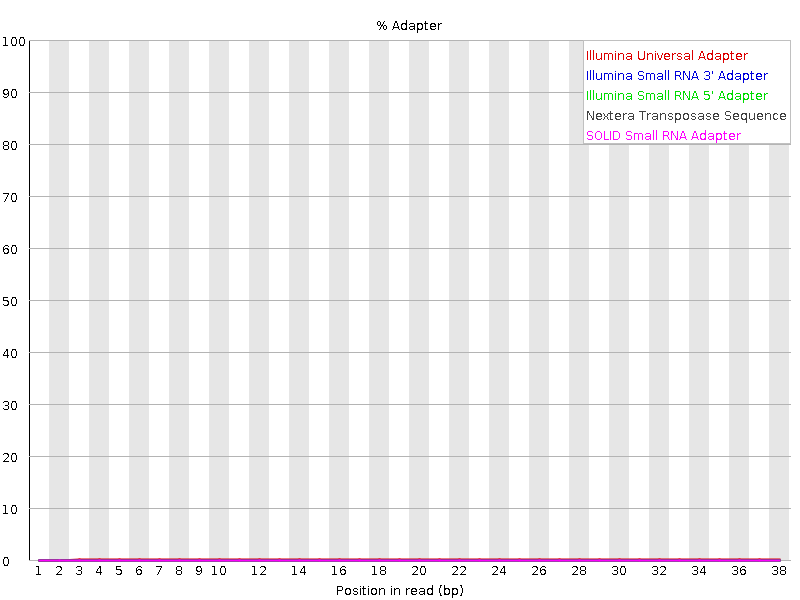
\includegraphics[width=0.8\textwidth]{img/SRR14325859_FastQC_Origin_img/adapter_content.png}	
	\caption{Adapter content\protect}    
\end{figure}

\begin{figure}[!htb]
	\centering
	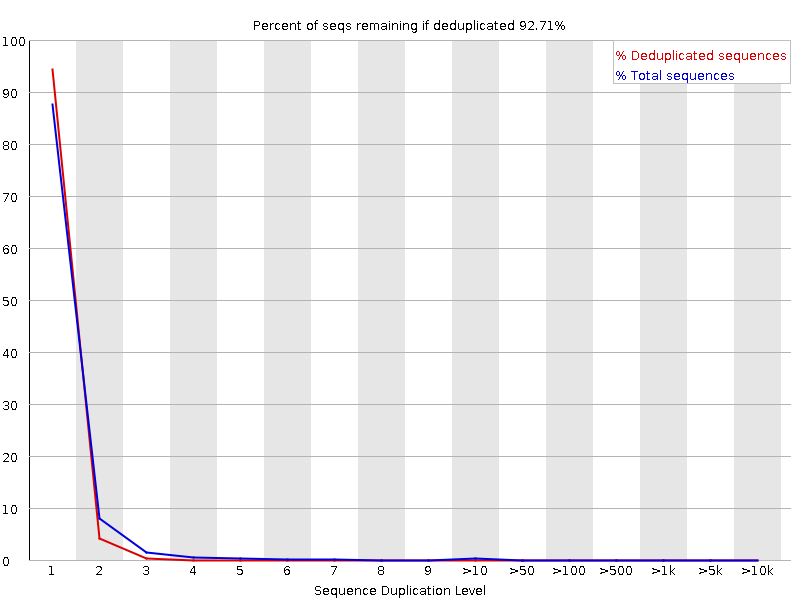
\includegraphics[width=0.8\textwidth]{img/SRR14325859_FastQC_Origin_img/duplication_levels.png}	
	\caption{Duplication levels\protect}    
\end{figure}

\begin{figure}[!htb]
	\centering
	\includegraphics[width=0.8\textwidth]{img/SRR14325859_FastQC_Origin_img/per_base_n_content.png}	
	\caption{Per base N content\protect}    
\end{figure}

\begin{figure}[!htb]
	\centering
	\includegraphics[width=0.8\textwidth]{img/SRR14325859_FastQC_Origin_img/per_base_quality.png}	
	\caption{Per base quality\protect}    
\end{figure}

\begin{figure}[!htb]
	\centering
	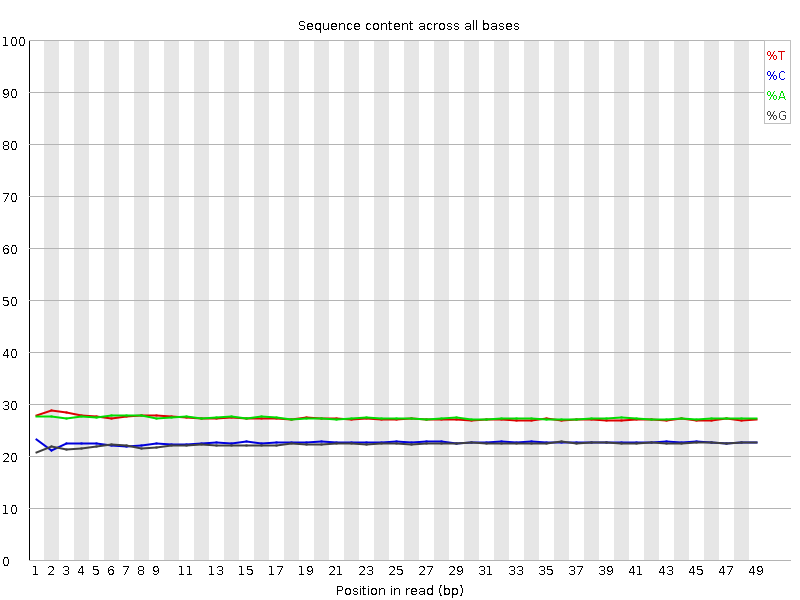
\includegraphics[width=0.8\textwidth]{img/SRR14325859_FastQC_Origin_img/per_base_sequence_content.png}	
	\caption{Per base sequence content\protect}    
\end{figure}

\begin{figure}[!htb]
	\centering
	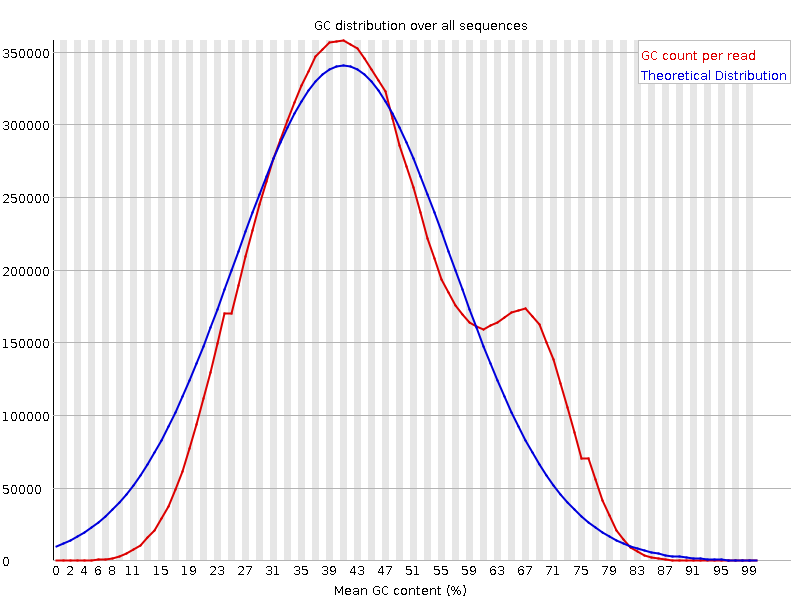
\includegraphics[width=0.8\textwidth]{img/SRR14325859_FastQC_Origin_img/per_sequence_gc_content.png}	
	\caption{Per sequence GC content\protect}    
\end{figure}

\begin{figure}[!htb]
	\centering
	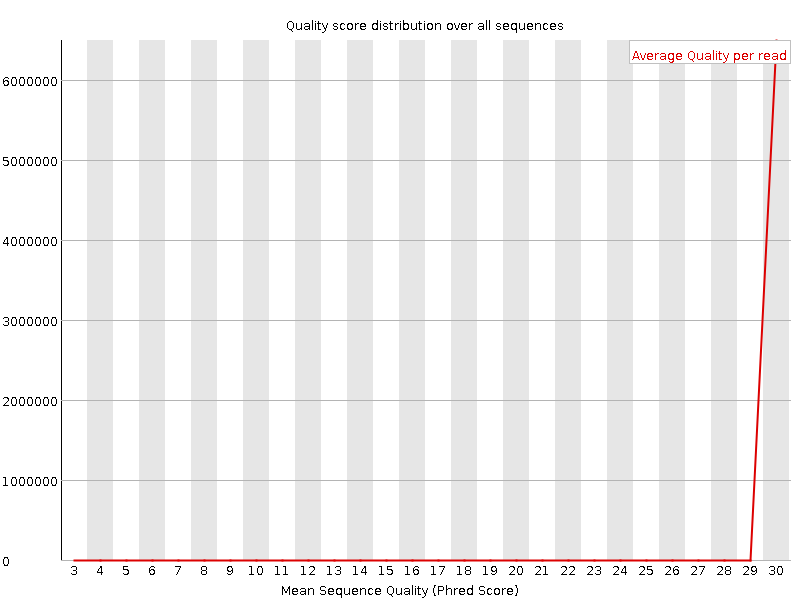
\includegraphics[width=0.8\textwidth]{img/SRR14325859_FastQC_Origin_img/per_sequence_quality.png}	
	\caption{Per sequence quality\protect}    
\end{figure}

\begin{figure}[!htb]
	\centering
	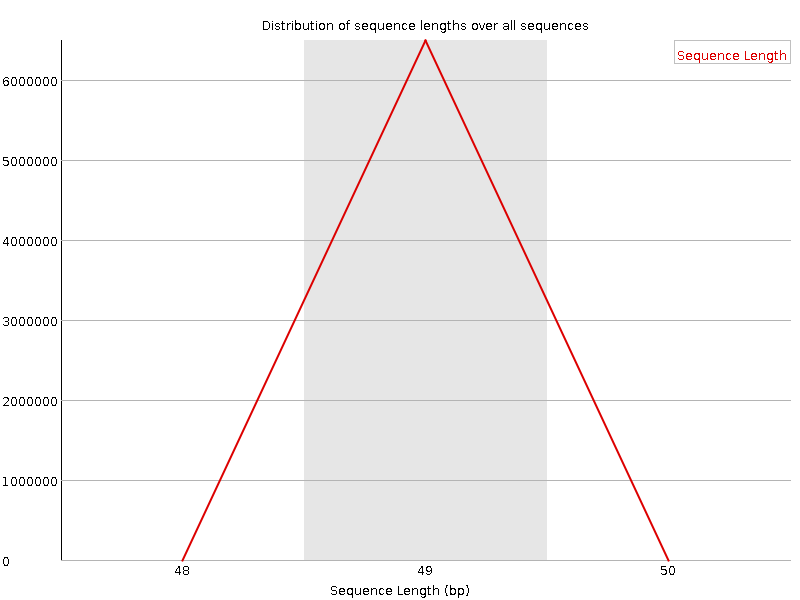
\includegraphics[width=0.8\textwidth]{img/SRR14325859_FastQC_Origin_img/sequence_length_distribution.png}	
	\caption{Sequence length distribution\protect}    
\end{figure}

\begin{figure}[!htb]
	\centering
	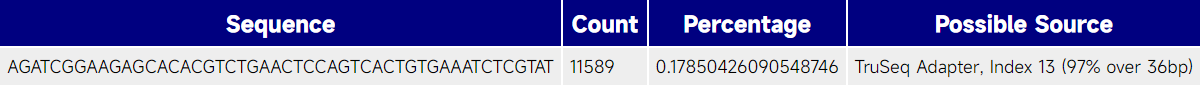
\includegraphics[width=0.8\textwidth]{img/SRR14325859_FastQC_Origin_img/overrepresented_sequences.png}	
	\caption{Overrepresented sequences\protect}    
\end{figure}



% \subsubsection{Processed Data}

\begin{figure}[!htb]
	\centering
	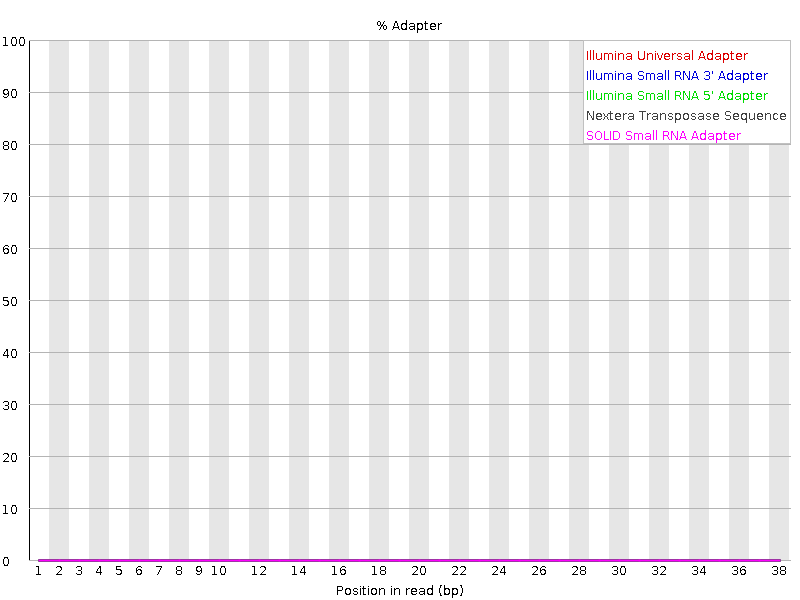
\includegraphics[width=0.8\textwidth]{img/SRR14325859_FastQC_Processed_img/adapter_content.png}	
	\caption{Adapter content (Processed)\protect}    
\end{figure}

\begin{figure}[!htb]
	\centering
	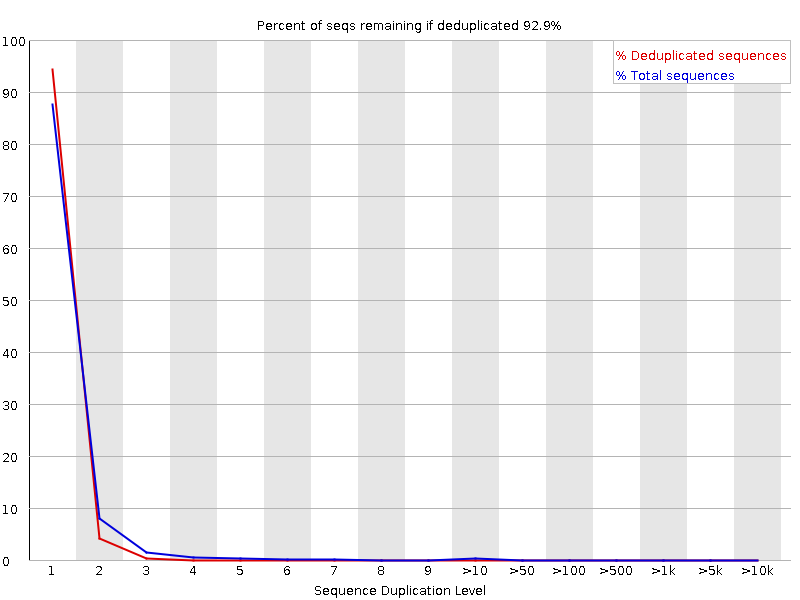
\includegraphics[width=0.8\textwidth]{img/SRR14325859_FastQC_Processed_img/duplication_levels.png}	
	\caption{Duplication levels (Processed)\protect}    
\end{figure}

\begin{figure}[!htb]
	\centering
	\includegraphics[width=0.8\textwidth]{img/SRR14325859_FastQC_Processed_img/per_base_n_content.png}	
	\caption{Per base N content (Processed)\protect}    
\end{figure}


\begin{figure}[!htb]
	\centering
	\includegraphics[width=0.8\textwidth]{img/SRR14325859_FastQC_Processed_img/per_base_quality.png}	
	\caption{Per base quality (Processed)\protect}    
\end{figure}

\begin{figure}[!htb]
	\centering
	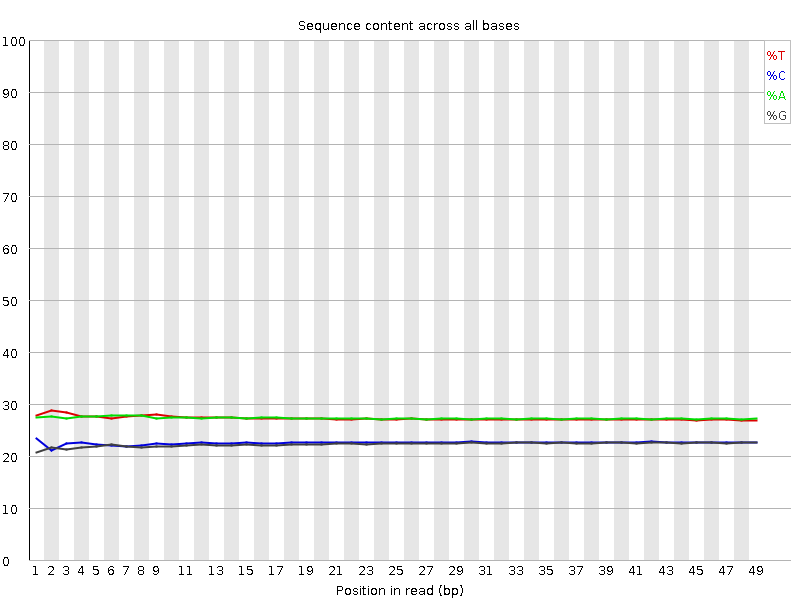
\includegraphics[width=0.8\textwidth]{img/SRR14325859_FastQC_Processed_img/per_base_sequence_content.png}	
	\caption{Per base sequence content (Processed)\protect}    
\end{figure}

\begin{figure}[!htb]
	\centering
	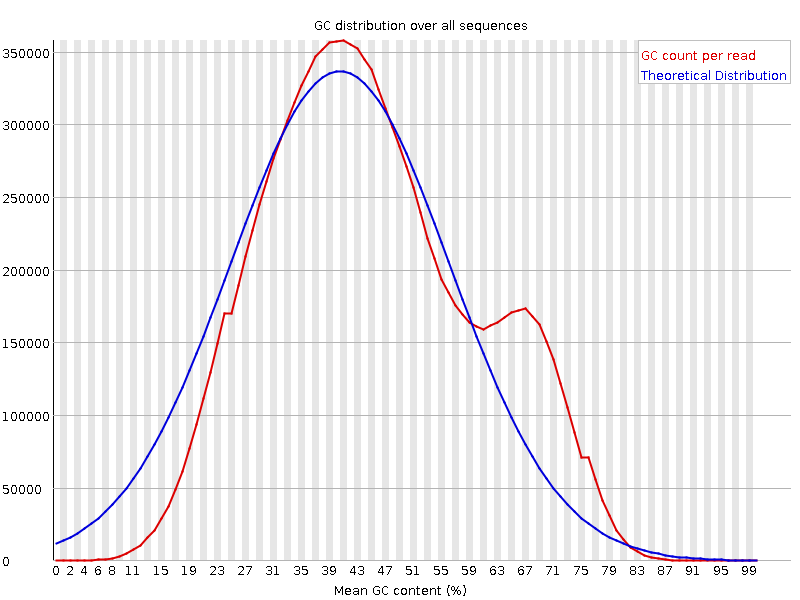
\includegraphics[width=0.8\textwidth]{img/SRR14325859_FastQC_Processed_img/per_sequence_gc_content.png}	
	\caption{Per sequence GC content (Processed)\protect}    
\end{figure}

\begin{figure}[!htb]
	\centering
	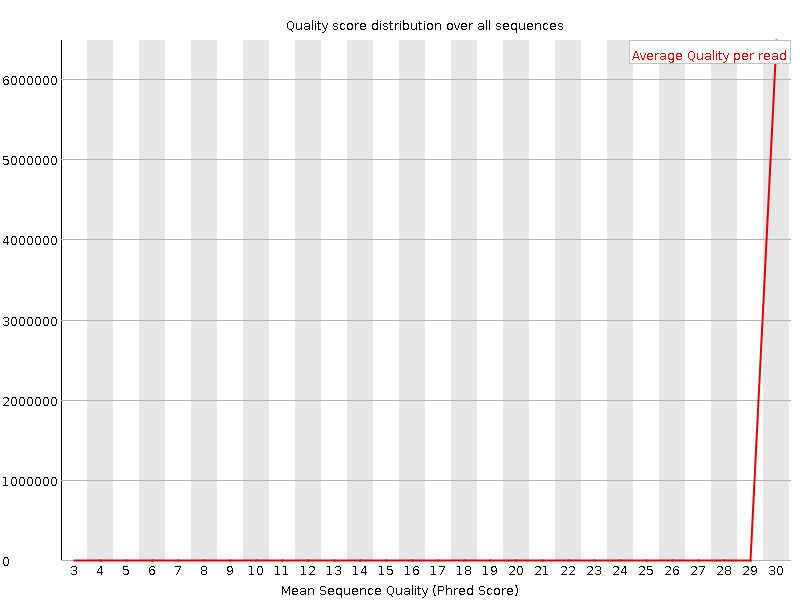
\includegraphics[width=0.8\textwidth]{img/SRR14325859_FastQC_Processed_img/per_sequence_quality.png}	
	\caption{Per sequence quality (Processed)\protect}    
\end{figure}

\begin{figure}[!htb]
	\centering
	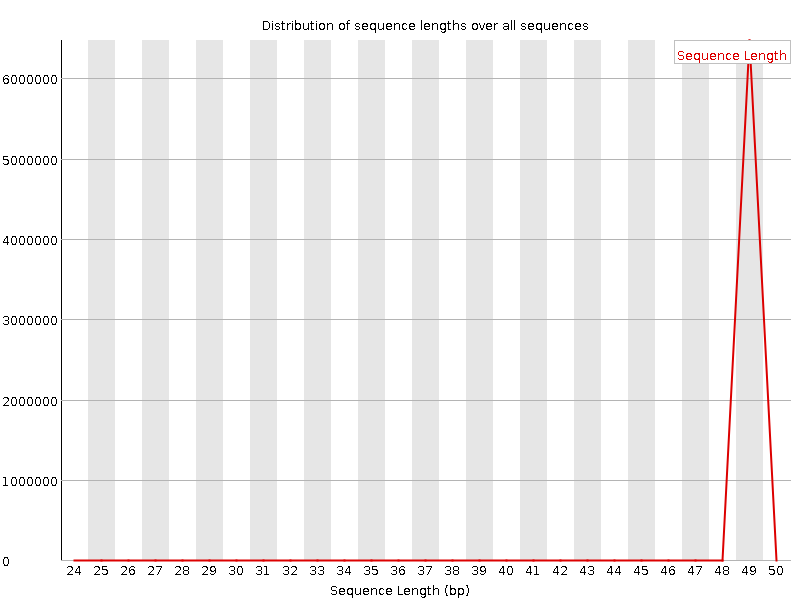
\includegraphics[width=0.8\textwidth]{img/SRR14325859_FastQC_Processed_img/sequence_length_distribution.png}	
	\caption{Sequence length distribution (Processed)\protect}    
\end{figure}

% \subsection{Peak calling}
\begin{figure}[h]
	\begin{minipage}{0.45\linewidth}
		\centerline{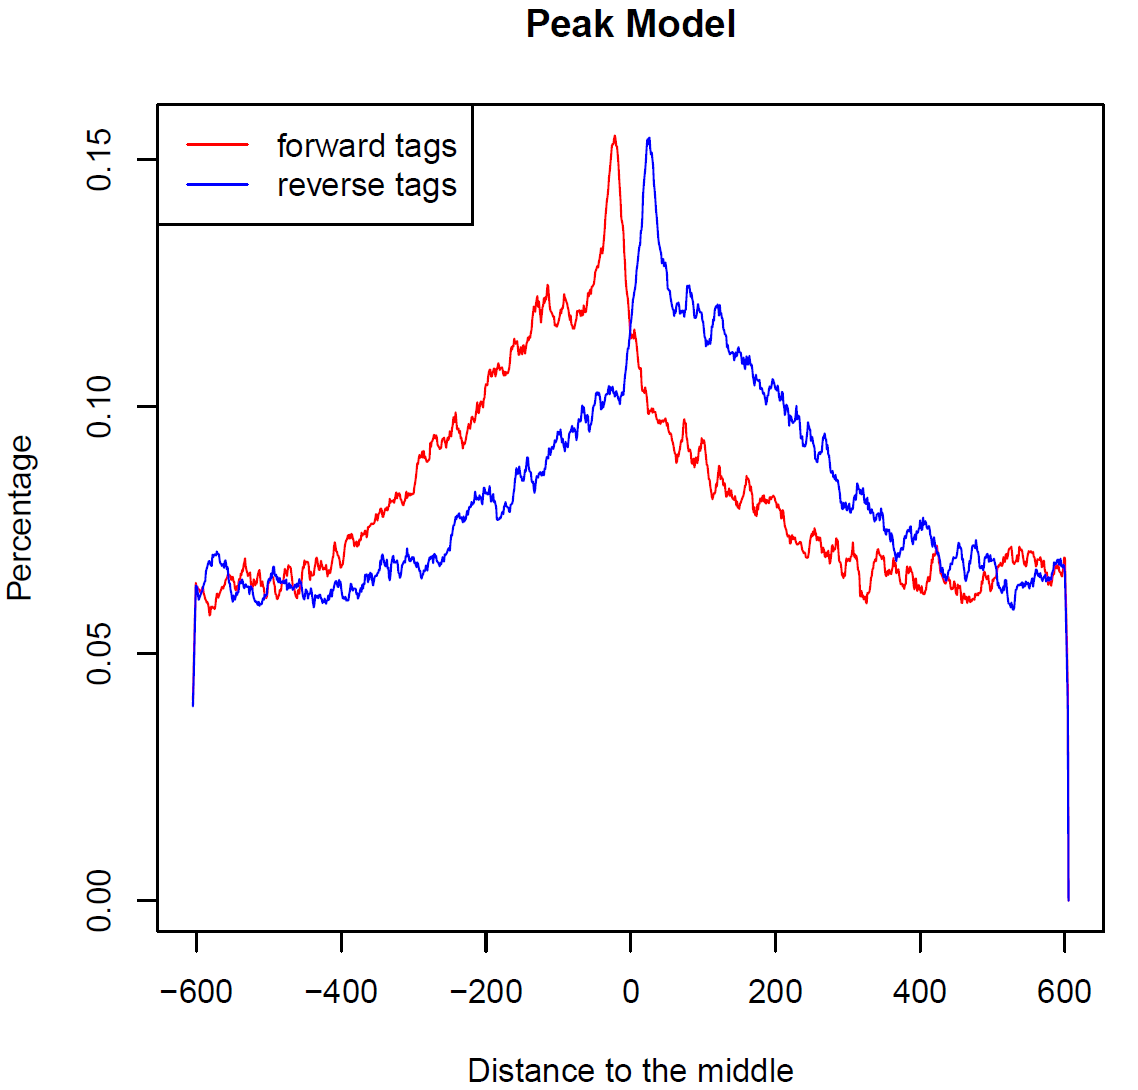
\includegraphics[width=\textwidth]{img/peak_model.png}}
		\centerline{Peak model}
	\end{minipage}
	\begin{minipage}{0.45\linewidth}
		\centerline{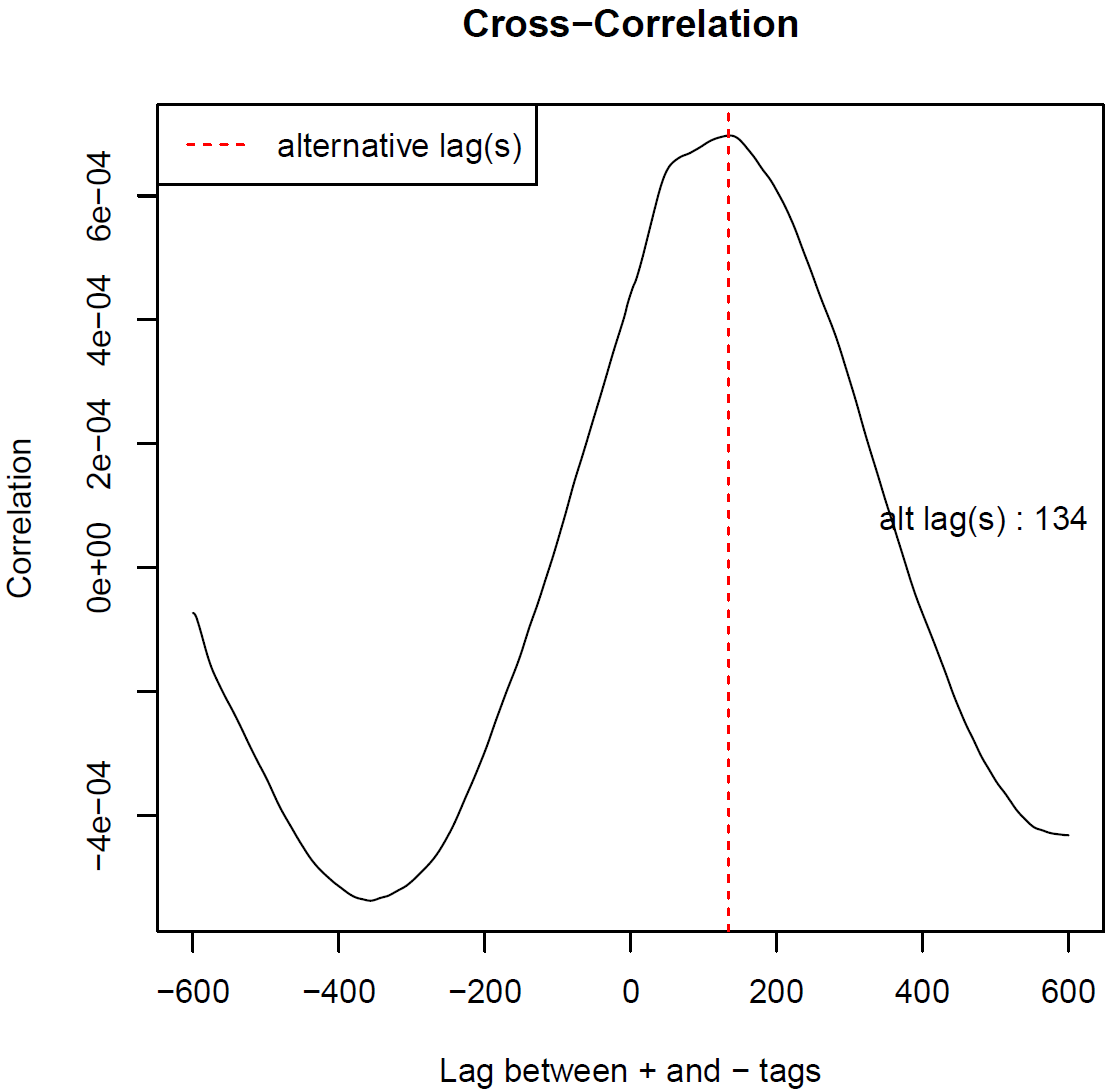
\includegraphics[width=\textwidth]{img/cross_correlation.png}}
		\centerline{Cross-Correlation}
\end{minipage}
\caption{Peak calling 结果}
\end{figure}

% \subsection{Motif Analysis}

\begin{figure}
	\centering
	\includegraphics[width=0.8\textwidth]{img/meme_out/logo1.eps}
\end{figure}

\begin{figure}
	\centering
	\includegraphics[width=0.8\textwidth]{img/meme_out/logo2.eps}
\end{figure}

\begin{figure}
	\centering
	\includegraphics[width=0.8\textwidth]{img/meme_out/logo3.eps}
	\caption{MEME 输出结果}
\end{figure}

% \subsection{Peak Annotation}

\begin{figure}[htb]
	\centering
	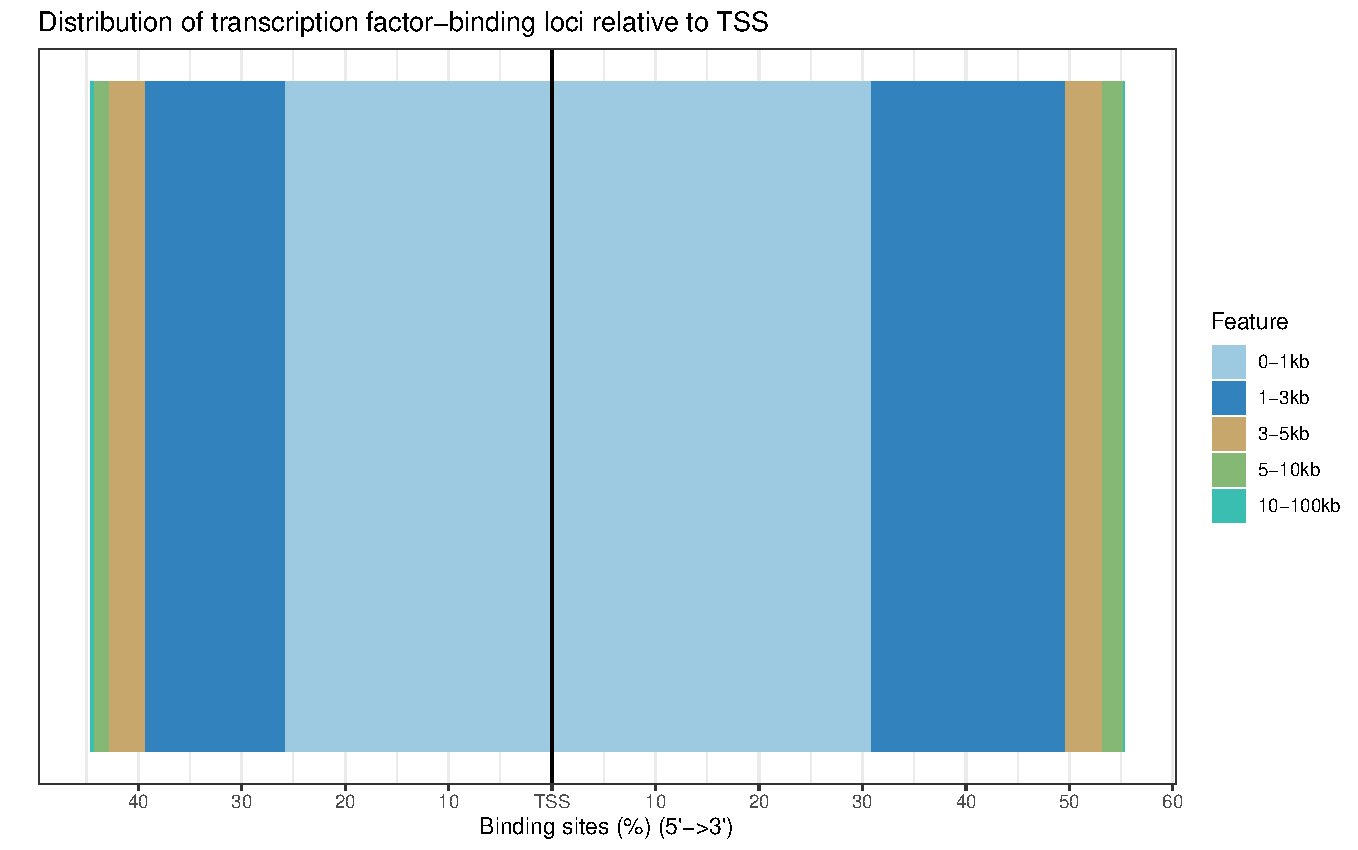
\includegraphics[width=\textwidth]{img/peak_distrubution.pdf}
    \caption{Distribution of transcription factor−binding loci relative to TSS}
\end{figure}

\begin{figure}
	\centering
	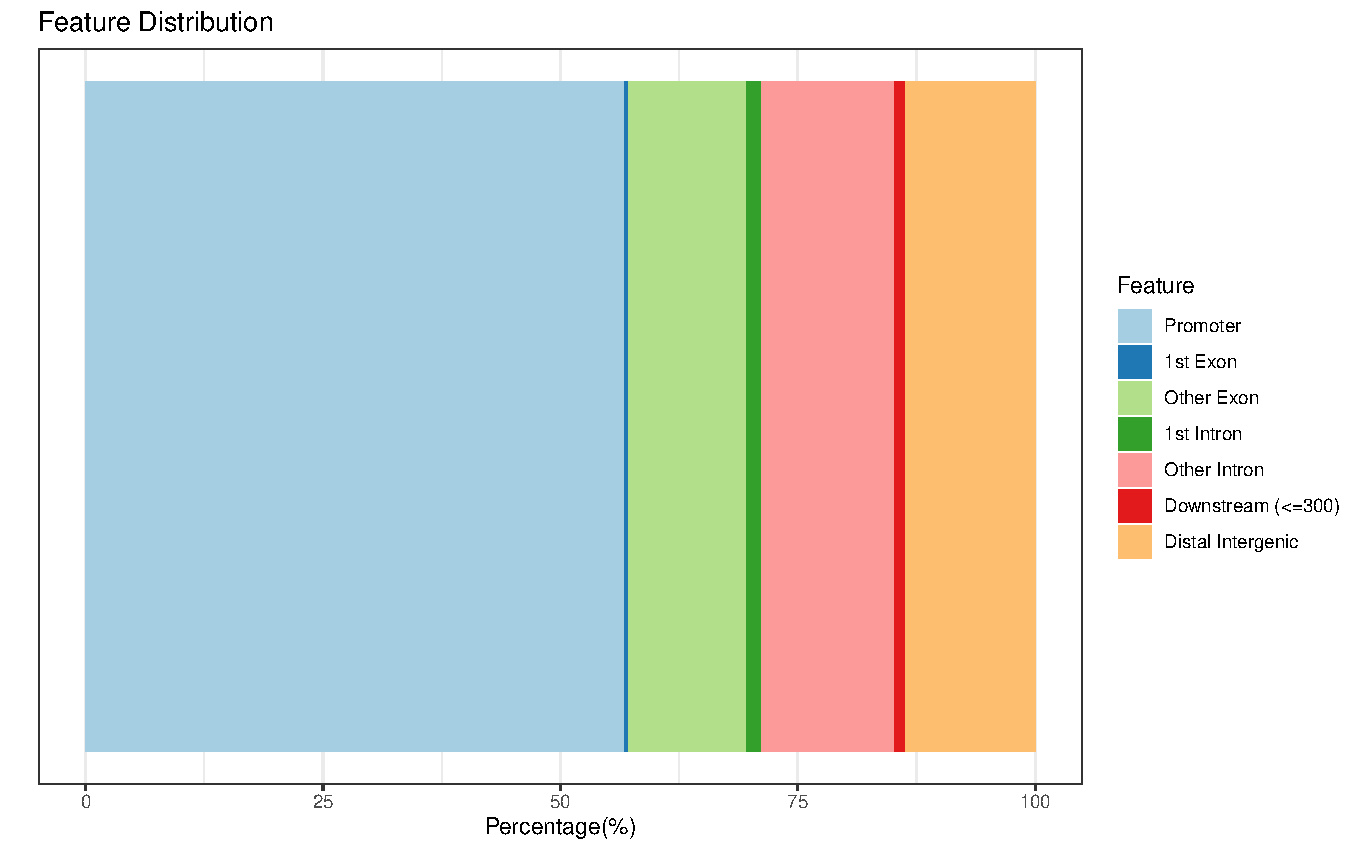
\includegraphics[width=\textwidth]{img/peaks_feature_distribution.pdf}
    \caption{Feature Distribution in Percentage}
\end{figure}

\begin{figure}
	\centering
	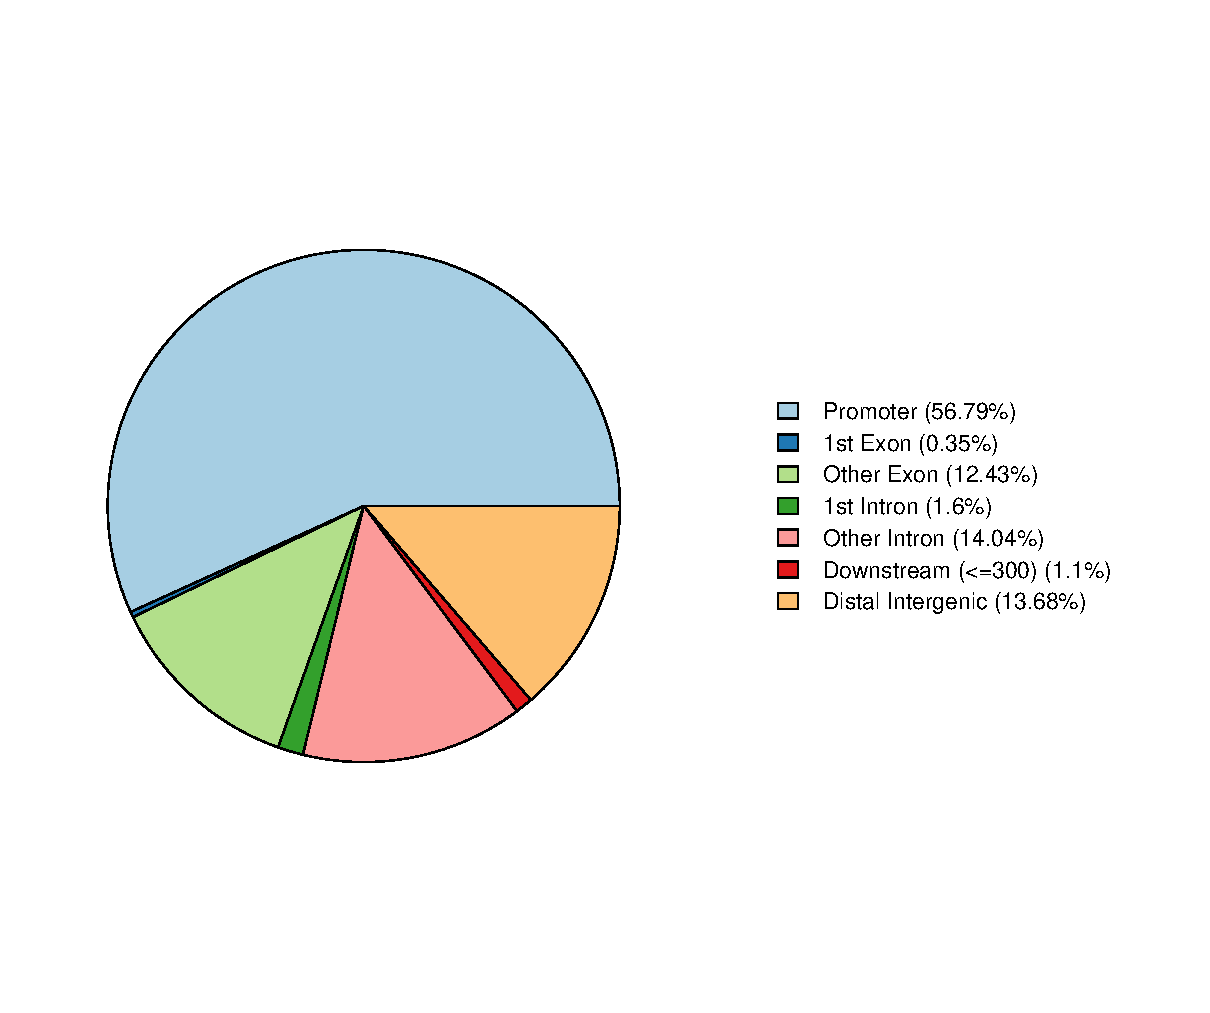
\includegraphics[width=0.8\textwidth]{img/peaks_pie.pdf}
    \caption{Feature Distribution in Pie Chart}
\end{figure}


% \subsection{Gene Ontology}

\begin{figure}[htb]
	\centering
	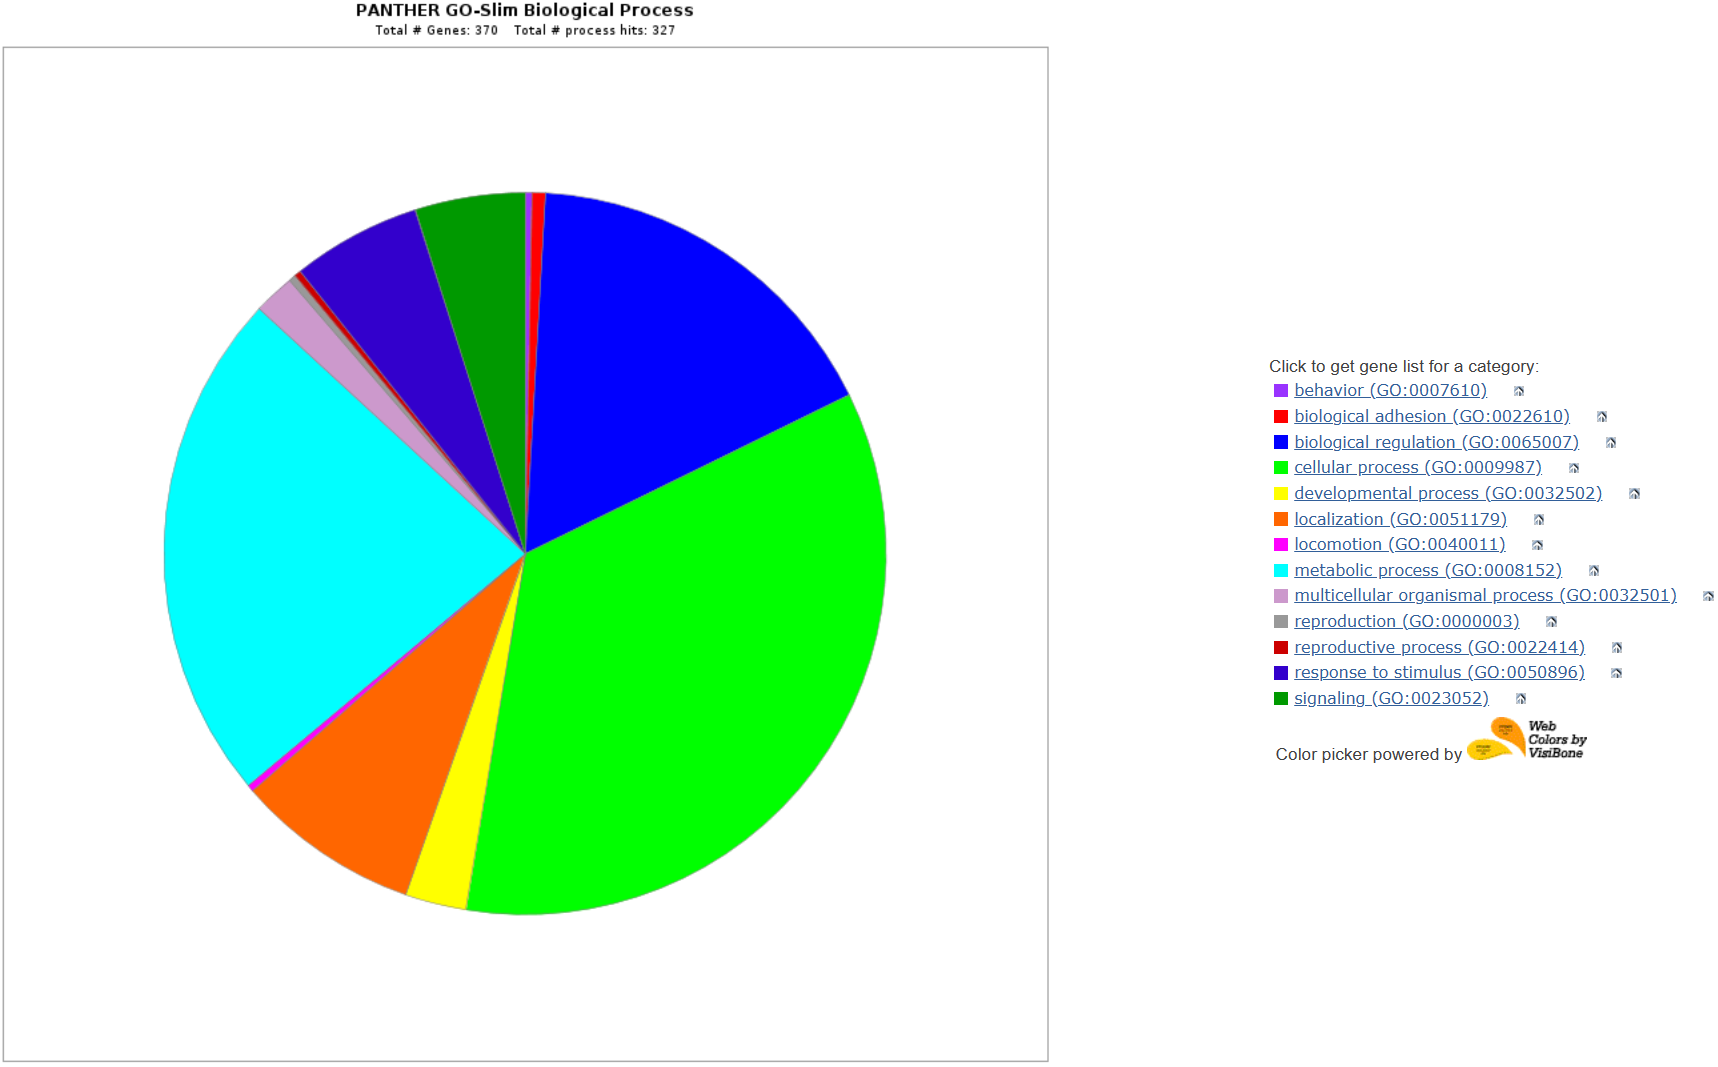
\includegraphics[width=0.8\textwidth]{img/GO_BioPro.png}
\end{figure}

\begin{figure}[h]
	\centering
	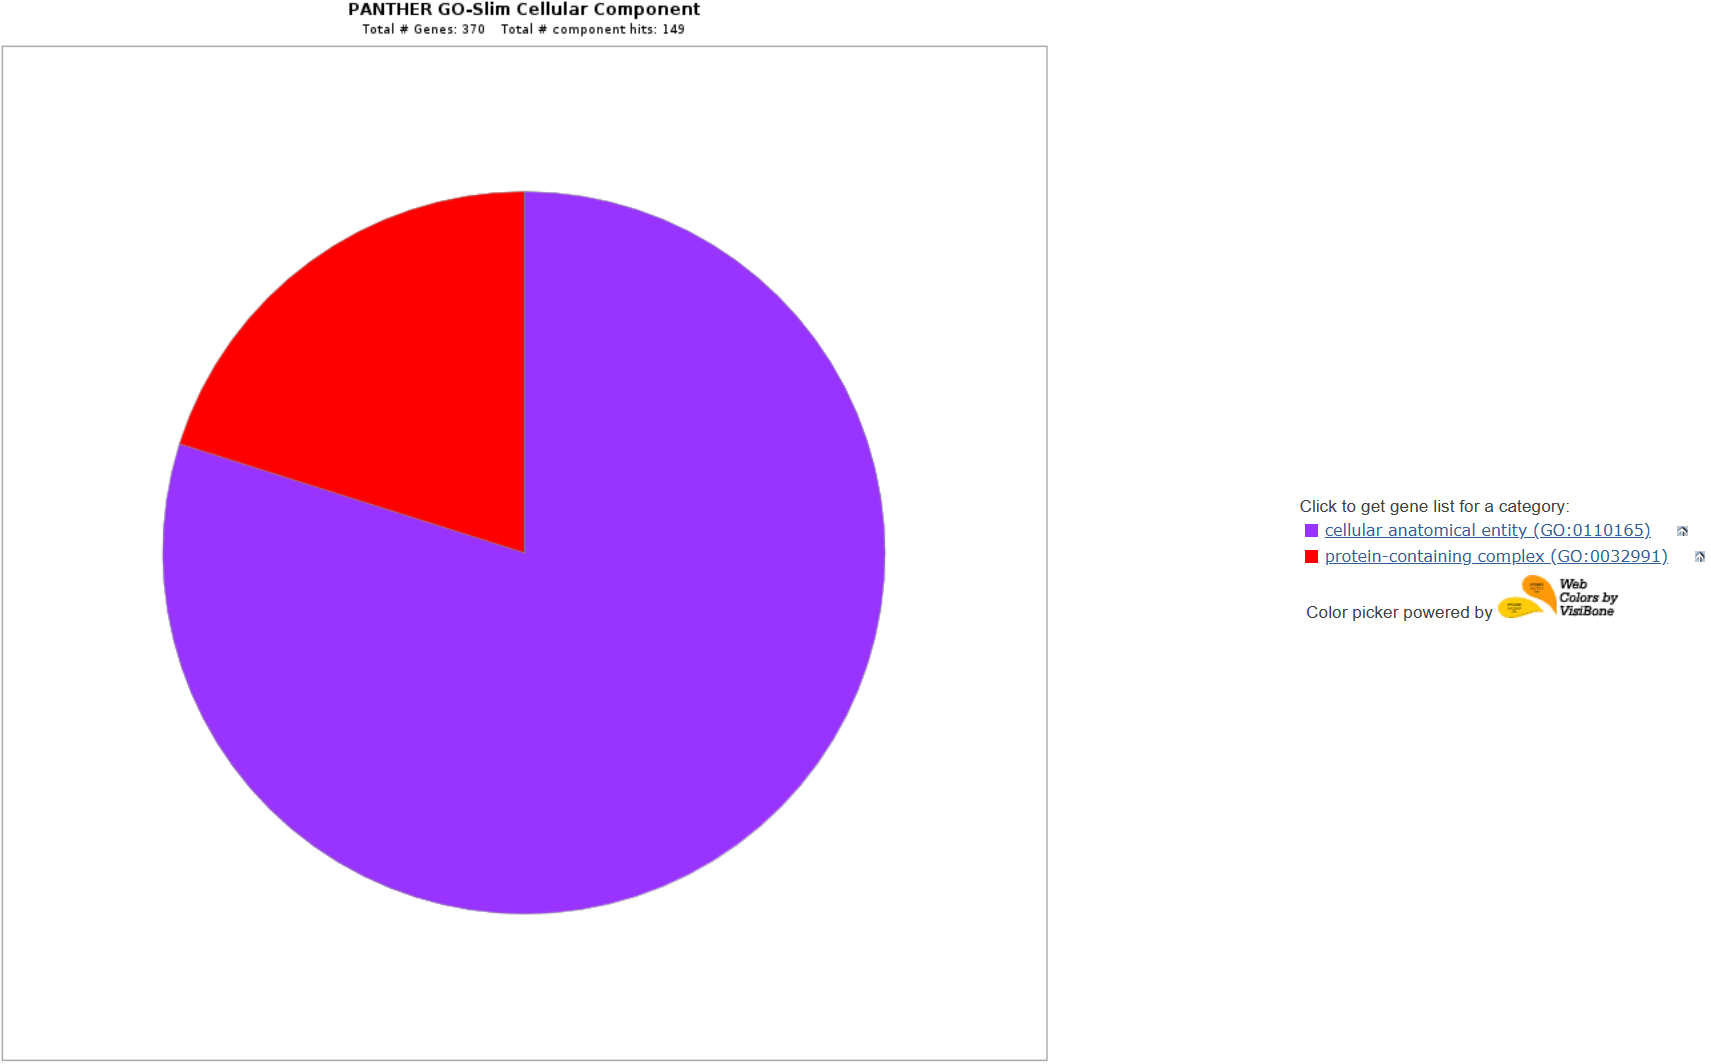
\includegraphics[width=0.8\textwidth]{img/GO_CelCom.png}
\end{figure}

\begin{figure}[h]
	\centering
	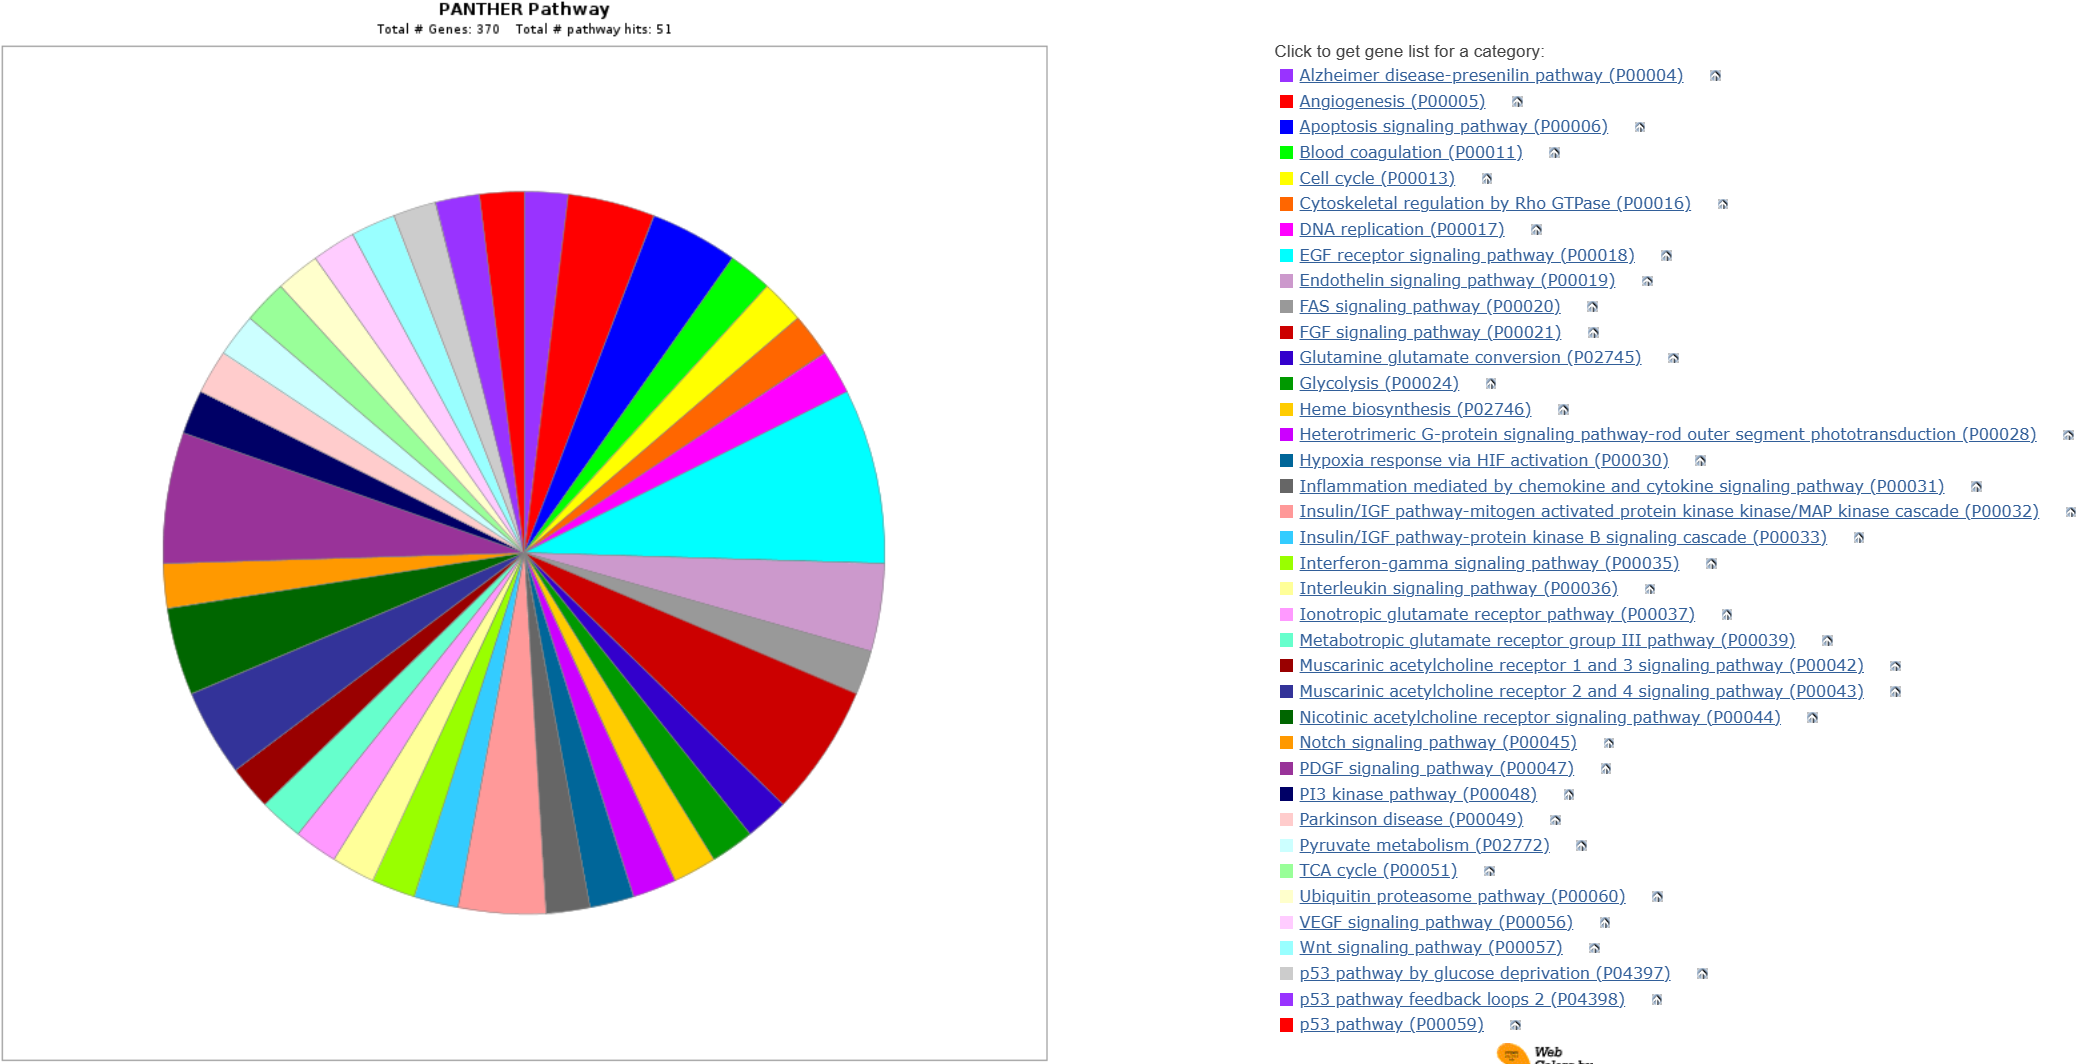
\includegraphics[width=\textwidth]{img/GO_Path.png}
\end{figure}

\begin{figure}[h]
	\centering
	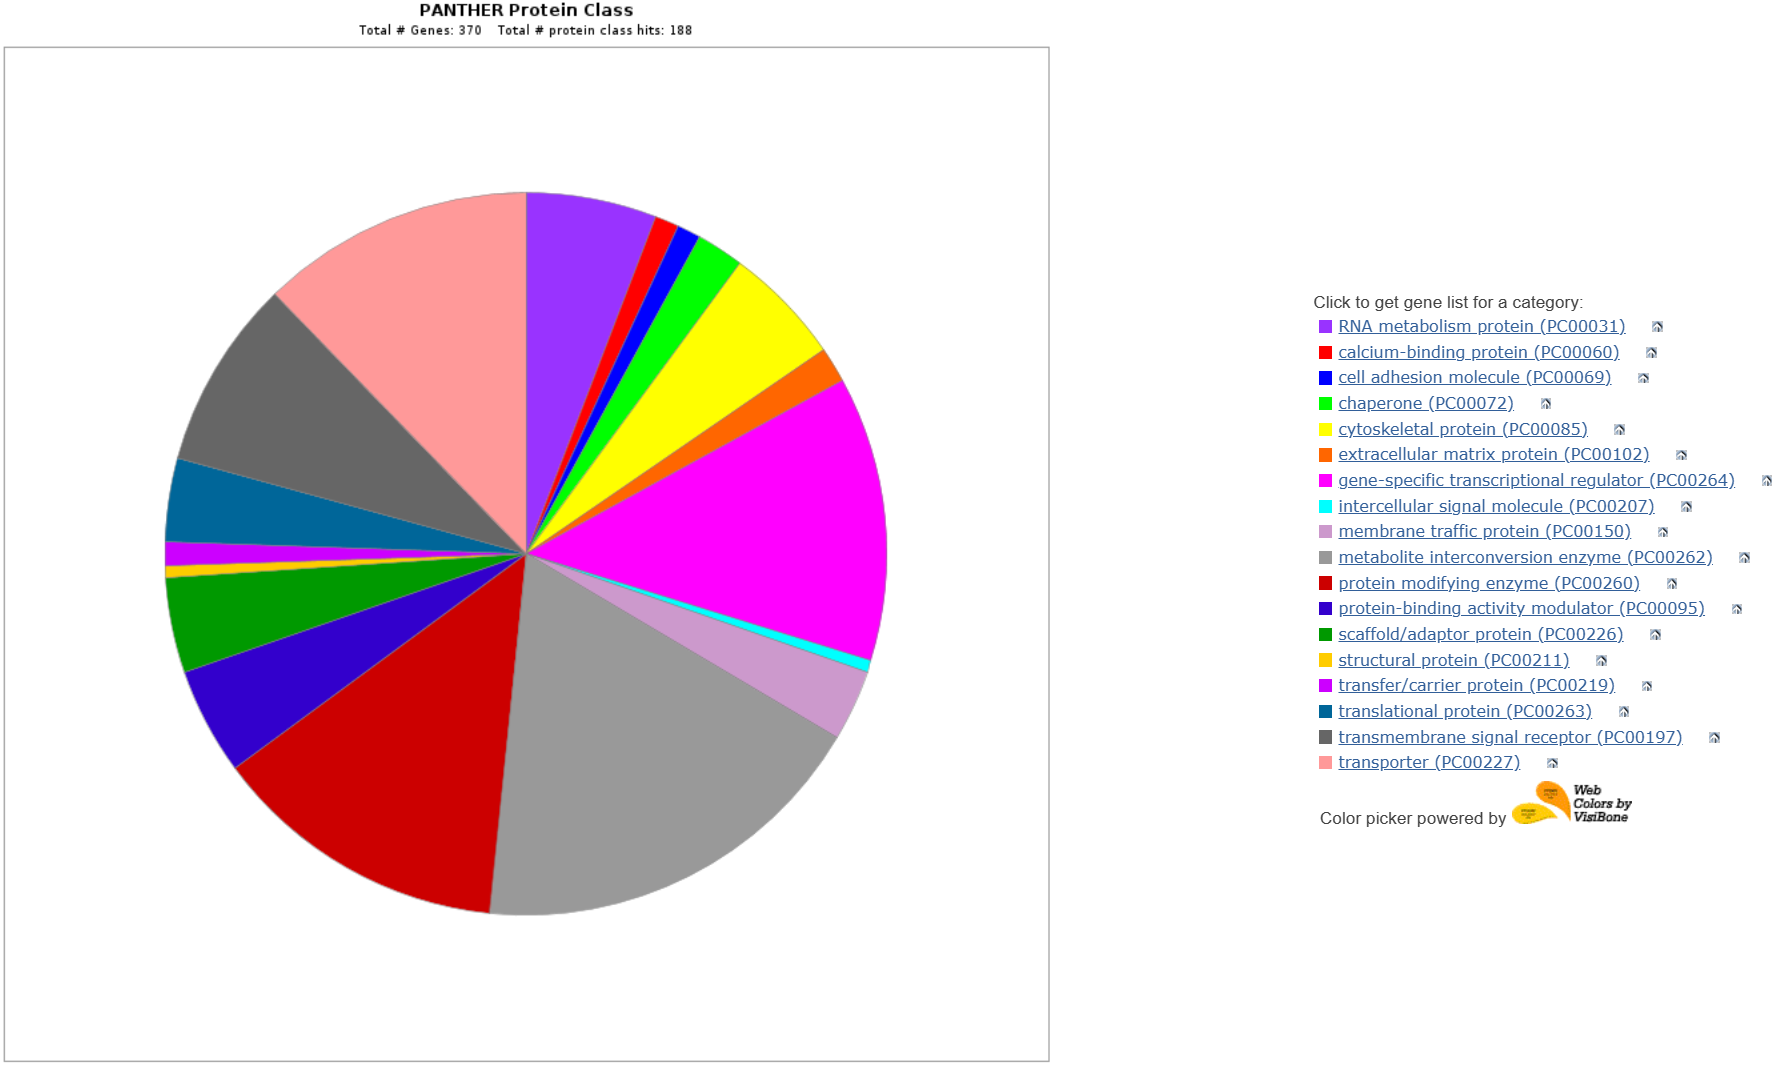
\includegraphics[width=\textwidth]{img/GO_ProCla.png}
\end{figure}

\begin{figure}[h]
	\centering
	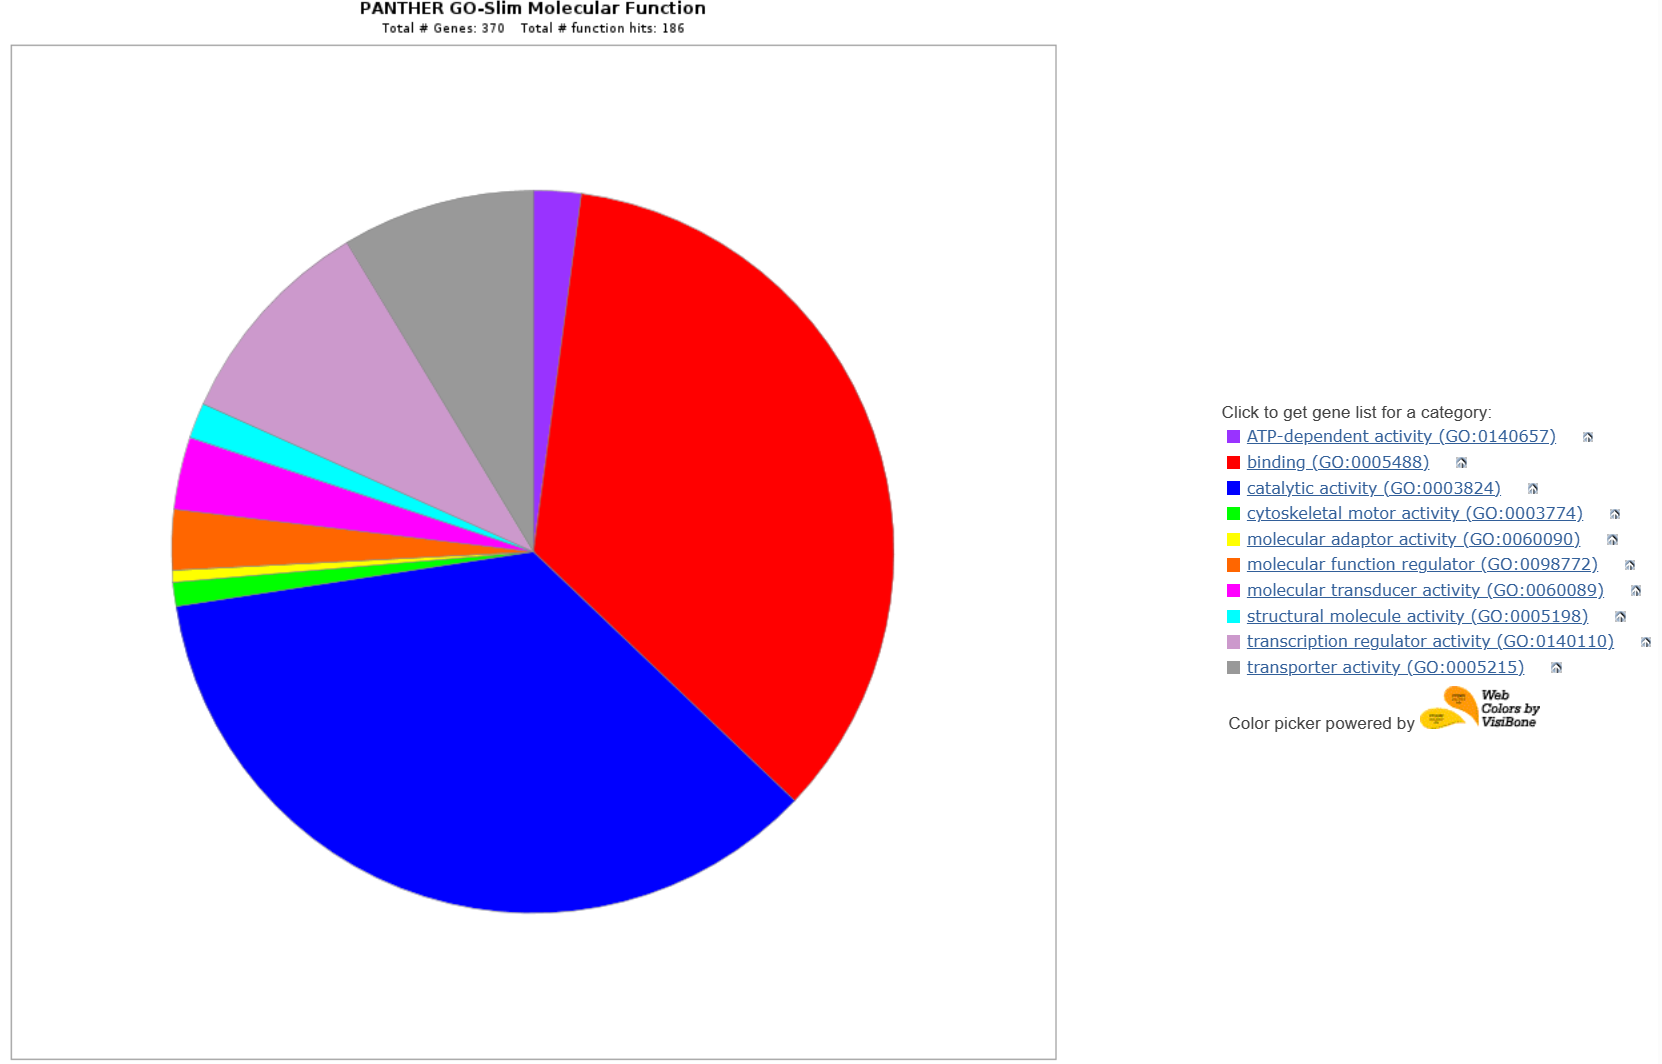
\includegraphics[width=\textwidth]{img/GO_MolFun.png}
\end{figure}

\clearpage

\section{讨论和结论}

文章\cite{ref1}的主要结论是,HIF-1(缺氧诱导因子1)可以促进PEP羧激酶(PCK-1)的表达,从而增加糖异生的速率,帮助线虫在缺氧和氧化应激下存活。文章\cite{ref1}使用了RNA-seq和ChIP-seq两种技术来分析缺乏HIF-1负调控因子EGL-9的突变体在有氧条件下的基因组、转录组和代谢组的变化。ChIP-seq是一种结合染色质免疫沉淀和高通量测序的方法,可以用来鉴定转录因子在基因组上的结合位点。文章\cite{ref1}利用ChIP-seq来确定HIF-1直接调控的基因,发现了200多个上调的基因,其中包括PEP羧激酶PCK-1。文章\cite{ref1}还验证了HIF-1结合到PCK-1启动子区域的特异性。ChIP-seq在文中\cite{ref1}的作用是揭示了HIF-1的转录调控网络,发现了一个新的HIF-1靶基因PCK-1,为研究HIF-1在糖异生中的作用提供了重要线索。

\clearpage

\begin{thebibliography}{99}

	\bibitem{ref1} Vora M, Pyonteck SM, Popovitchenko T, Matlack TL, Prashar A, Kane NS, Favate J, Shah P, Rongo C. The hypoxia response pathway promotes PEP carboxykinase and gluconeogenesis in C. elegans. Nat Commun. 2022 Oct 18;13(1):6168. doi: 10.1038/s41467-022-33849-x. PMID: 36257965; PMCID: PMC9579151.

\end{thebibliography}

\end{document}